\documentclass[a4paper,12pt]{article}
\usepackage[spanish]{babel} % Paquete para utilizar el español
\usepackage{palatino} % Para cambiar el tipo de letra
\usepackage{graphicx}

% Reconocimiento de caracteres del idioma Español en LaTeX.
\usepackage[utf8x]{inputenc} % Codificacion de entrada
\usepackage[T1]{fontenc} % Codificacion de fuente

% Cabecera de la "portada"
\title{\textbf{StickMotion:} Editor de posturas, posiciones y movimientos}
\author{\small\textit{Carmona Varo, Fernando; García García, José Manuel; López Fernandez, David;}\\
	\small\textit{Navas Torres, Francisco Javier; Porras Bueno, Javier}}

\begin{document}

  \maketitle % Crea el título y los autores

  \begin{abstract}
    El presente documento se corresponde con el entregable nº 2. El cliente recibirá el primer prototipo de la interfaz y a continuación se comenzará
    con la descripción de forma breve y detallada de la misma.\\
  \end{abstract}

  \section{Áreas de la interfaz}
  La aplicación principal consta de una serie de elementos o áreas principales, las cuales se reflejan en la figura \ref{interfaz} y son, de arriba 
  hacia abajo:
  \begin{figure} [h] \begin{center}
    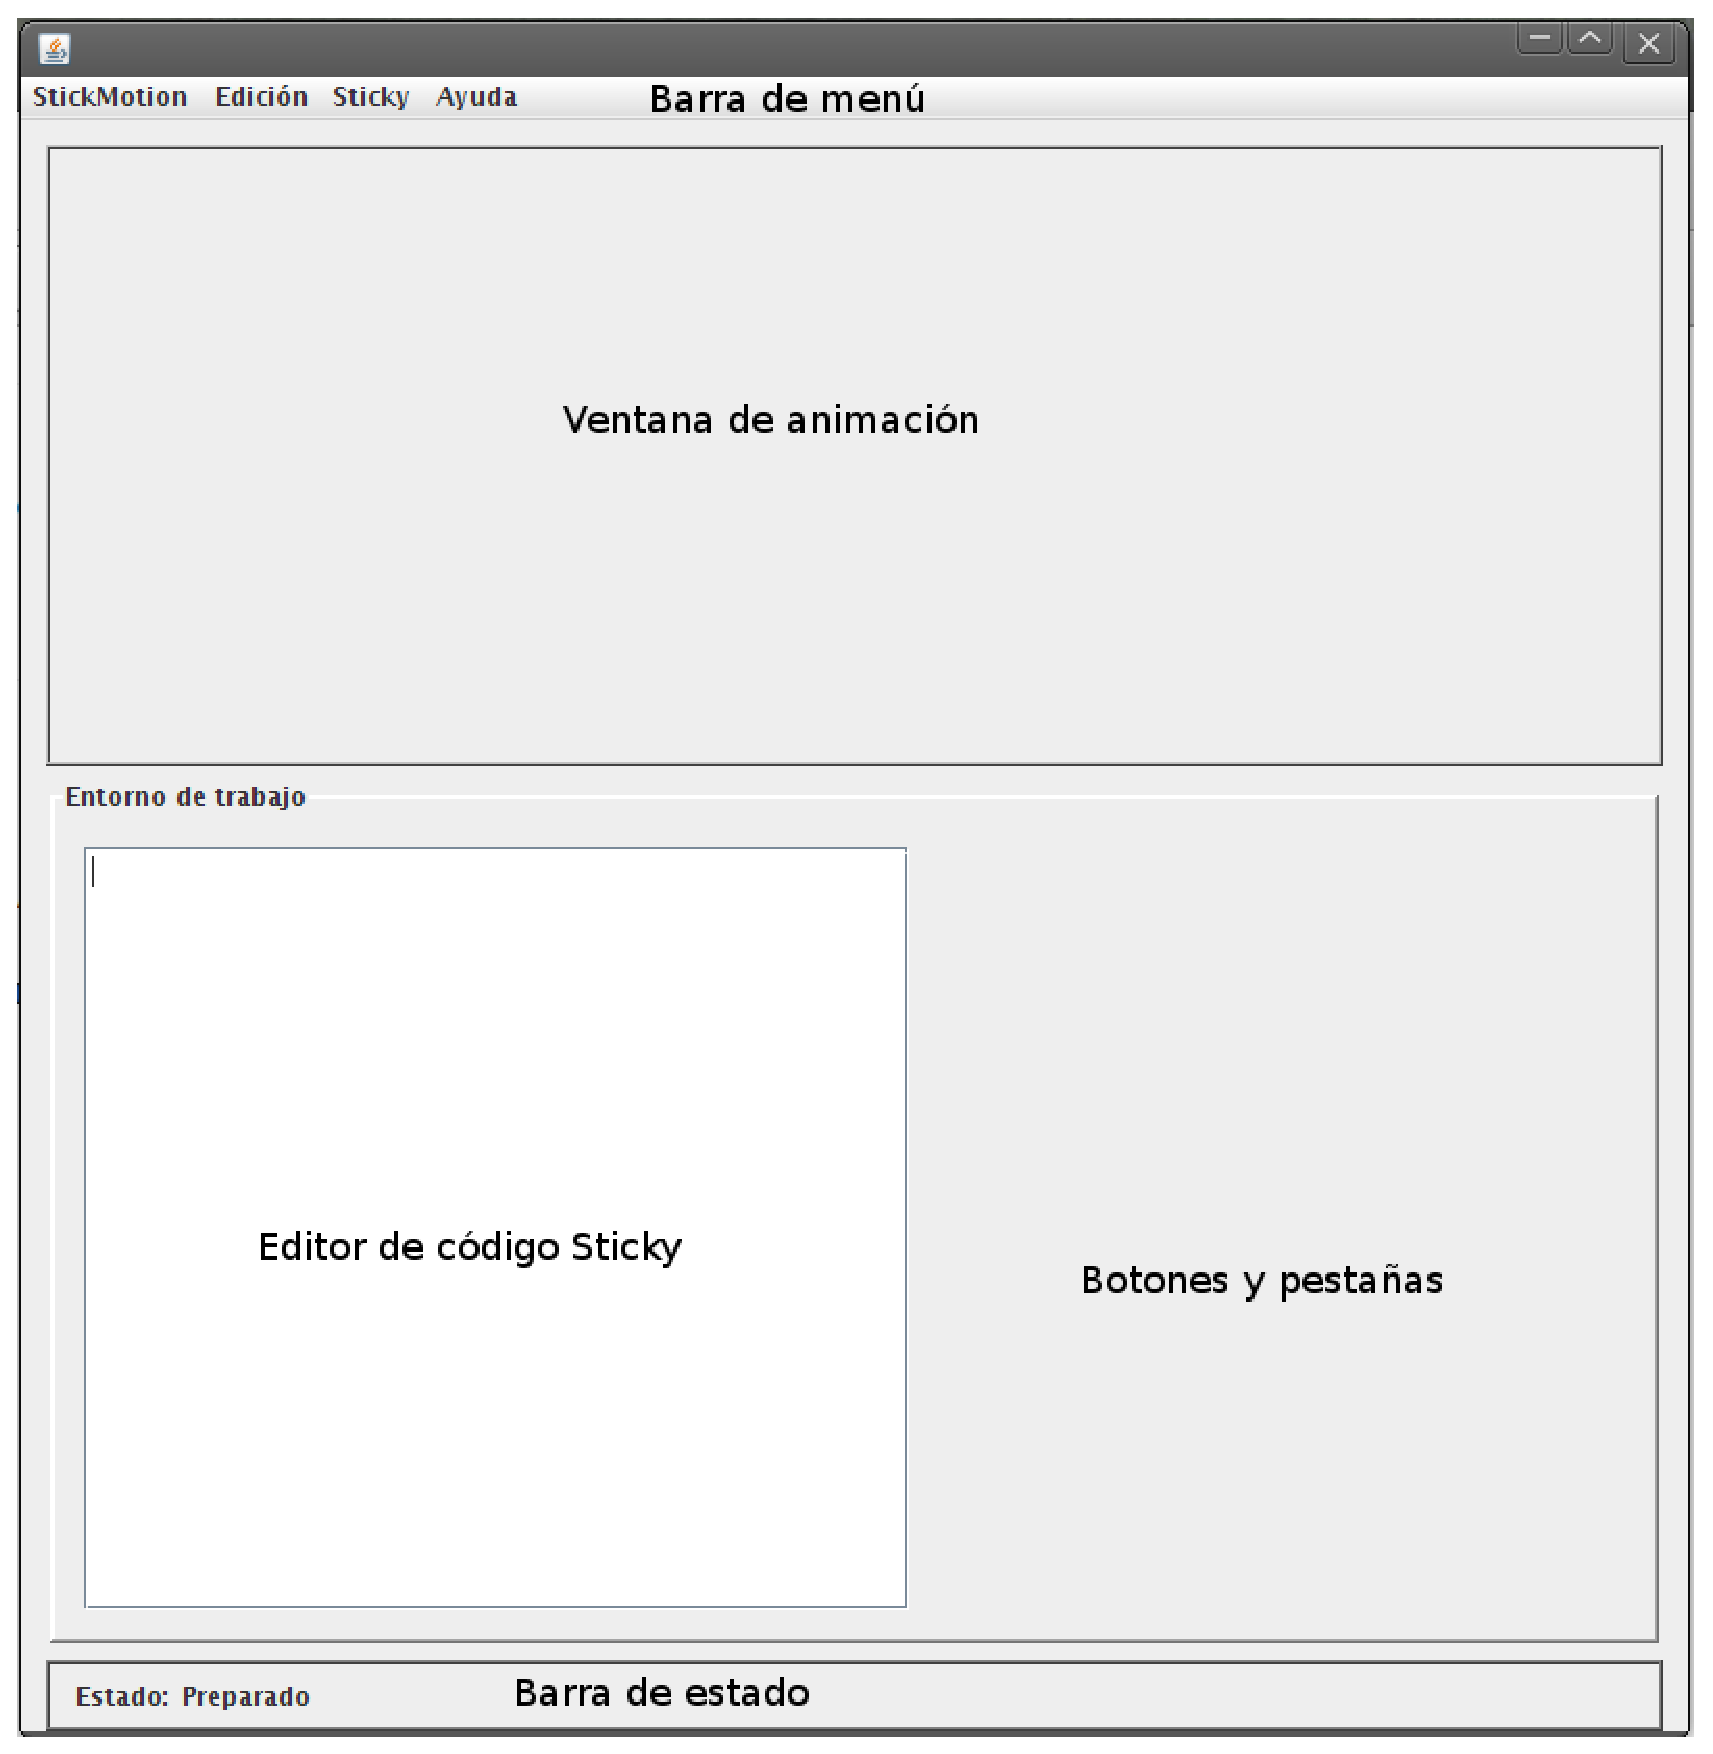
\includegraphics[height=0.95\textwidth]{AreasInterfazTexto}
    \caption{Áreas de la interfaz de la aplicación.} \label{interfaz}
  \end{center} \end{figure}
  \begin{itemize}
    \item \textbf{Barra de menú:} Será descrita con mayor profundidad más adelante.
    \item \textbf{Ventana de animación:} En este panel se mostrará al Stickman ejecutando las acciones que resulten de la interpretación del código
          fuente escrito por el usuario.
    \item \textbf{Editor de código \textbf{\textit{Sticky}}:} En este submenú aparecen todos los componentes del lenguaje \textbf{\textit{Sticky}}:
          operadores, bucles, condicionales, movimientos básicos, etc. que facilitan al usuario la escritura y desarrollo del código fuente mediante
          el editor de texto incorporado.
    \item \textbf{Botones y pestañas:} Este área aún está por definir, pero contendrá los botones, pestañas, atajos... que el usuario utilizará,
          presumiblemente, con mayor frecuencia, facilitando así el uso de la aplicación y mejorando la experiencia del usuario con la misma.
    \item \textbf{Barra de estado:} Mediante esta pequeña barra de estado se le informa al usuario en todo momento de lo que está ocurriendo en la
          aplicación. Puede mostrar mensajes aclarativos (como una descripción detallada de lo que cada opción del menú permite realizar, haciendo
          que la interfaz sea totalmente usable sin necesidad de acudir constantemente a la ayuda) o mensajes de acción (``limpiando el editor de
          texto''), entre otros.\\
  \end{itemize}

    \subsection{La barra de menú}
    La barra de menú está compuesta por las siguientes opciones, las cuales se detallan a continuación:
    \begin{itemize}
      \item \texttt{\textit{StickMotion:}} Contiene las opciones para crear un nuevo fichero fuente, guardar el actual o abrir uno nuevo. Además, 
            desde aquí se incluye la opción para salir de la aplicación (o usando el atajo de teclado correspondiente: \textit{CTRL + S}).
      \item \texttt{\textit{Edición:}} Contiene las opciones relacionadas con el editor de texto embebido en la aplicación con las típicas funciones
            de copiar, cortar y pegar.
      \item \texttt{\textit{Sticky:}} Contiene las opciones relativas al lenguaje \textbf{\textit{Sticky}}: bucles, condicionales, etc. de manera
            que se reduce el número de caracteres (normalmente bloques de código repetitivo) que debe escribir el usuario.
      \item \texttt{\textit{Ayuda:}} Contiene información acerca de la aplicación, del lenguaje \textbf{\textit{Sticky}} y sobre sus 
            desarrolladores.\\ 
    \end{itemize}
    También es importante destacar que todas las acciones que se pueden realizar desde el menú incorporan la combinación de teclas para establecer
    atajos de teclado. Aunque escapa fuera del ámbito de este documento, es necesario distinguir entre dos tipos de atajos: los de \textit{propósito
    general} y los de \textbf{\textit{Sticky}}.
\end{document}
